\documentclass{beamer}
\usepackage[utf8]{inputenc}
\usepackage[ngerman]{babel}
\usepackage{amsmath}
\usepackage{graphicx}
\usepackage{xcolor}
\usepackage{pdflscape}
\usepackage{color}
\usepackage{colortbl}
\usepackage{tabularx}
\usepackage{multirow}
\usepackage{algorithm}
\usepackage{algcompatible}
\usepackage{algorithmicx}
\usepackage{algpseudocode}
\usepackage{hyperref}
%\usepackage{utopia} %font utopia imported
%packages of house work
\usepackage{tabularray}
\usepackage{diagbox}
\usepackage{tikz}
\usetikzlibrary{shapes} 
\usepackage{pgfplots}
\usepackage{pgfplotstable}
\usepackage{tikz}
\usetikzlibrary{arrows.meta}
\usepackage{filecontents}
\usepackage[utf8]{inputenc}
\usepackage[ngerman]{babel}
%\usepackage[american]{babel}
\setcounter{secnumdepth}{4}
\usepackage{pdflscape}
\usepackage{lipsum}
\usepackage{mdwlist}
\usepackage{graphicx}
\usepackage{tabularx}
\usepackage{multirow}
\usepackage{rotating}
\usepackage{color}
\usepackage{colortbl}
\usepackage{multicol}
\usepackage{amsmath}
\usepackage{amsthm}
\usepackage{amssymb}
\usepackage{algorithm}
\usepackage{algcompatible}
\usepackage{algorithmicx}
\usepackage{algpseudocode}
\algblock[Class]{Class}{End}
\usepackage{wrapfig}
\usepackage{float}
\usepackage{url}
\usepackage{pdfpages}
\usepackage{cprotect}
\usepackage{setspace}
\usepackage{nomencl}
\usepackage{listings} 
\usepackage{cleveref}
\usepackage{rotating}
\usepackage{tikz}
\usepackage{adjustbox}
\usepackage{lscape}


\algrenewcommand\algorithmicrequire{\textbf{Input}}
\algrenewcommand\algorithmicensure{\textbf{Output}}
\renewcommand\algorithmiccomment[1]{\hfill$\triangleright\,$\textit{#1}}
\newcommand{\RNum}[1]{\uppercase\expandafter{\romannumeral #1\relax}}
\algrenewtext{Function}[2]{\algorithmicfunction\ \texttt{#1(#2)}}
\algnewcommand\algorithmicforeach{\textbf{for each}}
\algdef{S}[FOR]{ForEach}[1]{\algorithmicforeach\ #1\ \algorithmicdo}

\lstset{language=Python}
\lstset{frame=lines}
%\lstset{caption={Insert code directly in your document}}
%\lstset{label={lst:code_direct}}
%\lstset{basicstyle=\footnotesize}
\usepackage{xcolor}

\definecolor{codegreen}{rgb}{0,0.6,0}
\definecolor{codegray}{rgb}{0.5,0.5,0.5}
\definecolor{codepurple}{rgb}{0.58,0,0.82}
\definecolor{backcolour}{rgb}{0.95,0.95,0.92}

\usetheme{Madrid}
\usecolortheme{seahorse}

%------------------------------------------------------------
%This block of code defines the information to appear in the
%Title page
\title[Bachelorarbeit] %optional
{Das Wortproblem für kontextfreie Sprachen in subkubischer Zeit}

%\subtitle{Theorem von Simon}

\author[] % (optional)
{Ahmad Yassin}

\institute[] % (optional)
{
	Bachelorarbeit\\
}

\date\today

\AtBeginSection[]
{
	\begin{frame}<beamer>[noframenumbering]{Gliederung}
		\tableofcontents[currentsection]
	\end{frame}
}

\setbeamertemplate{bibliography item}{\insertbiblabel}


\begin{document}
	
	%The next statement creates the title page.
	\frame{\titlepage}
	\begin{frame}{Gliederung}
		\tableofcontents
	\end{frame}
	
	
	%---------------------------------------------------------
	
	
	\section{Einleitung}
	
	%---------------------------------------------------------
	%  Slide 1: Motivation 
	%---------------------------------------------------------
	
	\begin{frame}{Einleitung}
		\begin{block}{Wortproblem}
			Gegeben: Eine Grammatik $G = (S, \Sigma, N, P)$ und ein Wort $w$.
			\\Frage: $w \in L(G)$? wobei $L(G)$ beschreibt die Sprache, die durch $G$ erzeugt wird.
		\end{block}
		\pause
		\begin{itemize}
		\item Der Cocke-Younger-Kasami-Algorithmus (CYK) ist eines der effizientesten Algorithmen, der für das lösen des Wortproblems für kontextfreie Sprachen dient.\\
		\pause
		\item Die Zeitkomplexität von dem CYK-Algorithmus beträgt  $O(n^{3})$.\\
		\pause
		\item Gibt es Algorithmen die eine bessere Zeitkomplexität haben als der CYK-Algorithmus?\\
		\pause
		\item Ja, es gibt viele, jedoch werden wir in dieser Arbeit der Leslie-G.-Valiant-Algorithmus (LGV) betrachten mit einer Zeitkomplexität von $O(n^{2.81})$.
		\end{itemize}
	\end{frame}

	\begin{frame}{Ziel der Arbeit}
		\begin{itemize}
			\item Zu zeigen, dass der LGV-Algorithmus schneller ist als der CYK-Algorithmus\vspace*{0.3cm}
			\pause
			\item Dafür sollen die beiden Algorithmen implementiert werden\vspace*{0.3cm}
			\pause
			\item Kontextfreie Grammatiken ín Chomsky-Normalform umwandeln\vspace*{0.3cm}
			\pause
			\item Python Version 3.10\vspace*{0.3cm}
			\pause
			\item Die Zeiten von beiden Algorithmen auf dem Uni-Cluster messen\vspace*{0.3cm}
			\pause
			\item Schauen, ob der LGV-Algorithmus wirklich besser als der CYK-Algorithmus ist\vspace*{0.3cm}
		\end{itemize}
	\end{frame}
	
	%---------------------------------------------------------
	\section{Chomsky-Normalform}
		\begin{frame}{Chomsky-Normalform}
			%		Beide Algorithmen CYK und LGV bekommen als Eingabe eine kontextfreie Grammatik in Chomsky-Normalform.
			%		\pause
			\begin{definition}[\textbf{Chomsky-Normalform}]
				Eine kontextfreie Grammatik $G = (S, \Sigma, N, P)$ ist genau dann in Chomsky-Normalform, wenn ihre Produktionen in einer von zwei einfachen Formen vorliegen:
				\begin{enumerate}
					\item $A \to BC$, wobei $A,\ B \ und \ C$ jeweils nichtterminale Zeichen sind, d. h. in $N$ liegen,
					\item $A \to a$, wobei $A$ ein nichtterminales Zeichen ist und $a$ ein terminales Zeichen ist und in $\Sigma$ liegt. 
				\end{enumerate}
			\end{definition}
			\pause
			Die Umwandlung in Chomsky-Normalform geschieht in 4 Schritten:
			\pause
			\begin{itemize}
				\item Eliminierung von nutzlosen Zeichen
				\pause
				\item Eliminierung von $\varepsilon$-Produktionen
				\pause
				\item Eliminierung von Einheitsproduktionen
				\pause
				\item Umwandlung in Chomsky-Normalform
			\end{itemize}
		\end{frame}
		\begin{frame}{Eliminierung von nutzlosen Zeichen}
			Ein Zeichen $X$ für eine Grammatik $G = (S, \ \Sigma, \ N, \ P)$ wird als nutzlos bezeichnet, wenn keine Ableitung der Form $S \to^{*} \alpha X \beta \to^{*} w$ existiert.\\
			\pause
			Diese Zeichen werden in zwei Gruppen unterbracht:\\
			\pause
			\begin{enumerate}
				\item Die Gruppe der nicht-erzeugenden Zeichen
				\pause
				\item Die Gruppe der unerreichbaren Zeichen
			\end{enumerate} 
		\end{frame}
		\begin{frame}{Eliminierung von $\varepsilon$-Produktionen}
			Eine $\varepsilon$-Produktion ist eine Produktion der Form $A \to \varepsilon$ oder $A \to ^{*} \varepsilon$.\\
			\pause
			Die Eliminierung geschieht in zwei Schritten:
			\pause
			\begin{enumerate}
				\item Der erste Schritt besteht darin, dass alle eliminierbaren nichtterminalen Zeichen gesucht und sie in einer Menge zusammengefasst werden.
				\pause
				\item werden diese Produktionen anhand der Menge $N_{new}$, die der vorige Algorithmus bereitstellt, eliminiert.
			\end{enumerate} 
			
		\end{frame}
		\begin{frame}{Eliminierung von Einheitsproduktionen}
			Eine Einheitsproduktion ist eine Produktion der Form $A \to B$, wobei A und B nichtterminale Zeichen sind.
			\pause
			Diese Produktionen der Form $A \to B$ lassen sich nicht entfernen, allerdings durch eine Reihe von Regeln $A \to \alpha_1|\alpha_2|\ldots|\alpha_n$ ersetzen, die durch $B \to \alpha_1|\alpha_2|\ldots|\alpha_n$ abgeleitet werden.
			
		\end{frame}
		\begin{frame}{Umwandlung in Chomsky-Normalform}
			Grammatiken, die durch den letzten Schritte erfüllen, besitzen weder nutzlose Zeichen noch $\varepsilon$-Produktionen noch Einheitsproduktionen.\\
			\pause
			Solche Grammatiken zwei verschiedene Formen von Produktionen:
			\pause
			\begin{enumerate}
				\item $A \to a$, was bereit als Chomsky-Normalform-Produktion aufgenommen werden kann
				\pause
				\item $A \to \alpha_1, \alpha_2, \ldots ,\alpha_n$, wobei $\alpha_i$ ein nichtterminales oder terminales Zeichen und $n \leq 2$ ist
			\end{enumerate}
		\end{frame}
	
	\section{Cocke-Younger-Kasami-Algorithmus (CYK)}
	
	\begin{frame}{Funktionalität}
		\begin{itemize}
		\item Der CYK-Algorithmus funktioniert nach dem bottom-up-Prinzip, d. h. er versucht vom Wort $w$ auf das Startsymbol $S$ zurückzurechnen.
		\pause
		\item Bei dieser Art der Berechnung sucht der Algorithmus nach einem Teilstring im aktuellen Wort $w = \alpha_1 \alpha_2 \ldots \alpha_i \ldots \alpha_j\ldots \alpha_n$
		\pause
		\item dabei sollte der Teilstring mit dem Rumpf einer Regel in $P$ übereinstimmen. Wenn z.B. die Regel $X \to \alpha_i \ldots \alpha_j$ in $P$ liegt
		\pause
		\item dann wird es im aktuellen Wort ersetzt und wir erhalten das neue Wort $w = \alpha_1 \alpha_2 \ldots X \ldots \alpha_{n-(j-i)+1}$.
		\end{itemize}
	\end{frame}
	
	\begin{frame}[plain]
		$$L = \{ a^{i}b^{j}c^{k} \ | \ i <= j+k \}$$
		$$G = (S,\ \ \{ a, \ b, \ c \}, \ \{A,\ C,\ X,\ B,\ Y_1,\ Y_2,\ S\}, \ P )$$
		$$P=\{S \to SC\ |\ AB\ |\ AY_1\ |\ c\ |\ AY_2\ |\ b\ |\ XB\ |\ AC,$$ 
		$$Y_1 \to SC, $$ 
		$$ Y_2\to XB, $$ 
		$$ X\to AY_2\ |\ AB\ |\ XB\ |\ b,$$
		$$ A\to a,\ C\to c,\ B\to b\}$$
		\begin{figure}[ht]
			\begin{tikzpicture}[scale=0.75]
				\begin{scope}[every node/.style={circle,thick,draw}]
					\node (A) at (0,0) {$v_1$};
					\node (B) at (3,0) {$v_2$};
					\node (C) at (6,0) {$v_3$};
					\node (D) at (9,0) {$v_4$};
					\node (E) at (12,0) {$v_5$};
					\node (F) at (15,0) {$v_6$};
				\end{scope}
				
				\begin{scope}[>={Stealth[black]},
					every node/.style={fill=white,circle},
					every edge/.style={draw=red}]
					\path [->] (A) edge node {a} (B);
					\path [->] (B) edge node {a} (C);
					\path [->] (C) edge node {b} (D);
					\path [->] (D) edge node {b} (E);
					\path [->] (E) edge node {c} (F);
				\end{scope}
			\end{tikzpicture}
		\end{figure}
	\end{frame}

	\begin{frame}[plain]
		\begin{figure}[H]
			\begin{tikzpicture}[scale=0.75]
				\begin{scope}[every node/.style={circle,thick,draw}]
					\node (A) at (0,0) {$v_1$};
					\node (B) at (3,0) {$v_2$};
					\node (C) at (6,0) {$v_3$};
					\node (D) at (9,0) {$v_4$};
					\node (E) at (12,0) {$v_5$};
					\node (F) at (15,0) {$v_6$};
				\end{scope}
				
				\begin{scope}[>={Stealth[black]},
					every node/.style={fill=white,circle},
					every edge/.style={draw=red}]
					\path [->] (A) edge node {a} (B);
					\path [->] (B) edge node {a} (C);
					\path [->] (C) edge node {b} (D);
					\path [->] (D) edge node {b} (E);
					\path [->] (E) edge node {c} (F);
					
					\path [->] (A) edge [bend right=80] node {$A$} (B);%a%
					\path [->] (B) edge [bend right=80] node {$A$} (C);%a%
					\path [->] (C) edge [bend right=80] node {$S,B,X$} (D);%b%
					\path [->] (D) edge [bend right=80] node {$S,B,X$} (E);%b%
					\path [->] (E) edge [bend right=80] node {$S,C$} (F);%c%
					
					
					%			\path [->] (A) edge [bend right=70] node {$\emptyset$}(B);%aa%
					%			\path [->] (D) edge [bend right=70] node {$Y_1,S$}(E);%bc%
					%			\path [->] (B) edge [bend right=70] node {$S,X$}(C);%ab%
					%			\path [->] (C) edge [bend right=70] node {$S,X,Y_2$}(D);%bb%
				\end{scope}
			\end{tikzpicture}
		\end{figure}
	\end{frame}

	\begin{frame}[plain]
		\begin{figure}[H]
			\begin{tikzpicture}[scale=0.75]
				\begin{scope}[every node/.style={circle,thick,draw}]
					\node (A) at (0,0) {$v_1$};
					\node (B) at (3,0) {$v_2$};
					\node (C) at (6,0) {$v_3$};
					\node (D) at (9,0) {$v_4$};
					\node (E) at (12,0) {$v_5$};
					\node (F) at (15,0) {$v_6$};
				\end{scope}
				
				\begin{scope}[>={Stealth[black]},
					every node/.style={fill=white,circle},
					every edge/.style={draw=red}]
					\path [->] (A) edge node {a} (B);
					\path [->] (B) edge node {a} (C);
					\path [->] (C) edge node {b} (D);
					\path [->] (D) edge node {b} (E);
					\path [->] (E) edge node {c} (F);
					
					\path [->] (A) edge [bend right=80] node {$A$} (B);%a%
					\path [->] (B) edge [bend right=80] node {$A$} (C);%a%
					\path [->] (C) edge [bend right=80] node {$S,B,X$} (D);%b%
					\path [->] (D) edge [bend right=80] node {$S,B,X$} (E);%b%
					\path [->] (E) edge [bend right=80] node {$S,C$} (F);%c%
					
					\path [->] (B) edge [bend right=90] node {$S,X$}(D);%abb%
					\path [->] (B) edge [bend right=100] node {$S,X,Y_2$}(E);%abb%
					
				\end{scope}
			\end{tikzpicture}
		\end{figure}
	\end{frame}

	\begin{frame}[plain]
		\begin{figure}[H]
			\begin{tikzpicture}[scale=0.75]
				\begin{scope}[every node/.style={circle,thick,draw}]
					\node (A) at (0,0) {$v_1$};
					\node (B) at (3,0) {$v_2$};
					\node (C) at (6,0) {$v_3$};
					\node (D) at (9,0) {$v_4$};
					\node (E) at (12,0) {$v_5$};
					\node (F) at (15,0) {$v_6$};
				\end{scope}
				
				\begin{scope}[>={Stealth[black]},
					every node/.style={fill=white,circle},
					every edge/.style={draw=red}]
					\path [->] (A) edge node {a} (B);
					\path [->] (B) edge node {a} (C);
					\path [->] (C) edge node {b} (D);
					\path [->] (D) edge node {b} (E);
					\path [->] (E) edge node {c} (F);
					
					\path [->] (A) edge [bend right=80] node {$A$} (B);%a%
					\path [->] (B) edge [bend right=80] node {$A$} (C);%a%
					\path [->] (C) edge [bend right=80] node {$S,B,X$} (D);%b%
					\path [->] (D) edge [bend right=80] node {$S,B,X$} (E);%b%
					\path [->] (E) edge [bend right=80] node {$S,C$} (F);%c%
					
					\path [->] (B) edge [bend right=90] node {$S,X$}(D);%abb%
					\path [->] (B) edge [bend right=90] node {$S,X,Y_2$}(E);%abb%
					\path [->] (A) edge [bend right=95] node {$S,X$}(E);%abb%
					\path [->] (A) edge [bend right=100] node {$S$}(F);%aabbc%
					
				\end{scope}
			\end{tikzpicture}
		\end{figure}
	\end{frame}
	


	\begin{frame}{CYK-Algorithmus in pseudocode}
		Der CYK-Algorithmus könnte in pseudocode wie folgt aussehen:	
		\begin{block}{CYK-Algorithmus}
			Sei eine Grammatik $G$ in CNF und ein Wort $w=a_1 \ldots a_n \in \Sigma^*$.\\
			(i) for $\mathrm{i}:=1$ to $\mathrm{n}$ do\\
			\ \ \ \ \ \ \ \ \ \ $\mathrm{V}_{\mathrm{i}, \mathrm{i}}:=\left\{\mathrm{A} \in \mathrm{V} \mid \mathrm{A} \rightarrow \mathrm{a}_{\mathrm{i}} \in \mathrm{R}\right\}$\\
			(ii) for $h:=1$ to $\mathrm{n}-1$ do\\
			\ \ \ \ \ \ \ \ \ \ \ \ for $i:=1$ to $n-h$ do\\
			\ \ \ \ \ \ \ \ \ \ \ \ \ \ \ \ \ \ $\mathrm{V}_{\mathrm{i}, \mathrm{i}+\mathrm{h}}=\bigcup_{j=i}^{i+h-1} V_{i, j} \cdot \mathrm{~V}_{j+1, i+h}$\\
			(iii) if $S \in \mathrm{V}_{1, \mathrm{n}}$\\
			\ \ \ \ \ \ \ \ \ \ then Ausgabe $\mathrm{w} \in \mathrm{L}(\mathrm{G})$\\
			\ \ \ \ \ else\\
			\ \ \ \ \ \ \ \ \ \  Ausgabe w $\notin \mathrm{L}(\mathrm{G})$
		\end{block}
	\end{frame}

	\begin{frame}{CYK-Algorithmus in pseudocode}
		Die Definition der Operation $\cdot$ ist wie folgt definiert:
		\begin{block}{\textbf{$N_1 \ \cdot \ N_2$}}
			Sei $ G = (S, \Sigma, N, P)$ eine Kontextfreie Grammatik in Chomsky Normalform und seien $N_1,N_2 \subseteq N$, dann gilt:
			$$N_1 \ \cdot \ N_2 = \{A \ |\ \exists  B\in N_1 , \exists C\in N_2 : A\to BC \in P\}$$
		\end{block}
	\end{frame}


	\begin{frame}{Komplexitätzeit und Implementierung}
		\begin{algorithm}[H]
			\floatname{algorithm}{Algorithmus}
			\setstretch{1.1}
			\caption[Teil (i)]{Teil (i)}
			\label{algorithm9}
			\begin{algorithmic}[1]
				\For{\texttt{$i:=1 \ to \ n$}}  \ \ \ \ \ \ \ \ \ \ \ \ \ \ \ \ \ \ \ \ \ \ \ \ \ \ \ \ \ \ \ \ \ \ \ \ \ \ \ \ \ \ \textbf{$ \%O(n)$ Durchläufe}
				\ForEach { $A\to\alpha \in P$} \ \ \ \ \ \ \ \ \ \ \ \ \ \ \ \ \ \ \ \ \ \ \ \ \ \ \ \ \textbf{$\%O(|P|)$ Durchläufe}
				\If{$A\to\alpha = B \to w_i$}
				\State Füge $A$ zur Menge des Listenelements $L_{[i,i]}$
				\Else
				\State Abbruch (Das Wort $w$ ist nicht ableitbar)
				\EndIf
				\EndFor
				\EndFor
			\end{algorithmic}
		\end{algorithm}
	\end{frame}

	\begin{frame}{Komplexitätzeit und Implementierung}
		\begin{algorithm}[H]
			\floatname{algorithm}{Algorithmus}
			\setstretch{1.1}
			\caption[Teil (ii)]{Teil (ii)}
			\label{algorithm10}
			\begin{algorithmic}[1]
				\For{\texttt{$h:=1 \ to \ n$}} \ \ \ \ \ \ \ \ \ \ \ \ \ \ \ \ \ \ \ \ \ \ \ \ \ \ \ \ \ \ \ \ \ \ \ \ \ \ \ \ \ \ \textbf{$ \%O(n)$ Durchläufe}
				\For{\texttt{$i:=1 \ to \ n-h$}} \ \ \ \ \ \ \ \ \ \ \ \ \ \ \ \ \ \ \ \ \ \ \ \ \ \ \ \ \ \ \ \ \ \textbf{$ \%O(n)$ Durchläufe}
				\For{\texttt{$j:=i \ to \ i+h-1$}} \ \ \ \ \ \ \ \ \ \ \ \ \ \ \ \ \ \ \ \ \ \ \ \ \textbf{$ \%O(n)$ Durchläufe}
				\ForEach { $A\to\alpha \in P$} \ \ \ \ \ \ \ \ \ \ \ \ \ \ \ \ \ \ \ \ \textbf{$\%O(|P|)$ Durchläufe}
				\If{$|\alpha| = 2 \land  \alpha_1 \in L_{[i,j]} \land  \alpha_2 \in L_{[j+1,i+h]}$}
				\State Füge $A$ zur Menge des Listenelements $L_{[i,i+h]}$
				\EndIf
				\EndFor
				\EndFor
				\EndFor
				\EndFor
			\end{algorithmic}
		\end{algorithm}
		 \href{http://www.cip.ifi.lmu.de/~lindebar/}{CYK-Algorithmus Funktionalität durch graphische Effekte}.
	\end{frame}
	
	%---------------------------------------------------------
	
	
	\section{Leslie-G.-Valiant-Algorithmus (LGV)}
	
	
	
	\begin{frame}{Leslie-G.-Valiant-Algorithmus (LGV)}
		durch eine Reihe von Reduktionen gezeigt, dass das Wortproblem für kontextfreie Sprachen im Bezug auf die Länge des Worts $n=|w|$ mindestens so schnell durchgeführt werden kann wie die Multiplikation für $n \times n$ boolesche Matrizen. Unter Verwendung der Strassen-Matrix-Multiplikation kann ein indirekter Algorithmus für das Wortproblem von Kontextfreien Sprachen abgeleitet werden, der eine Zeitkomplexität von $O(n^{2.81})$ hat.
		\begin{figure}
			\centering
			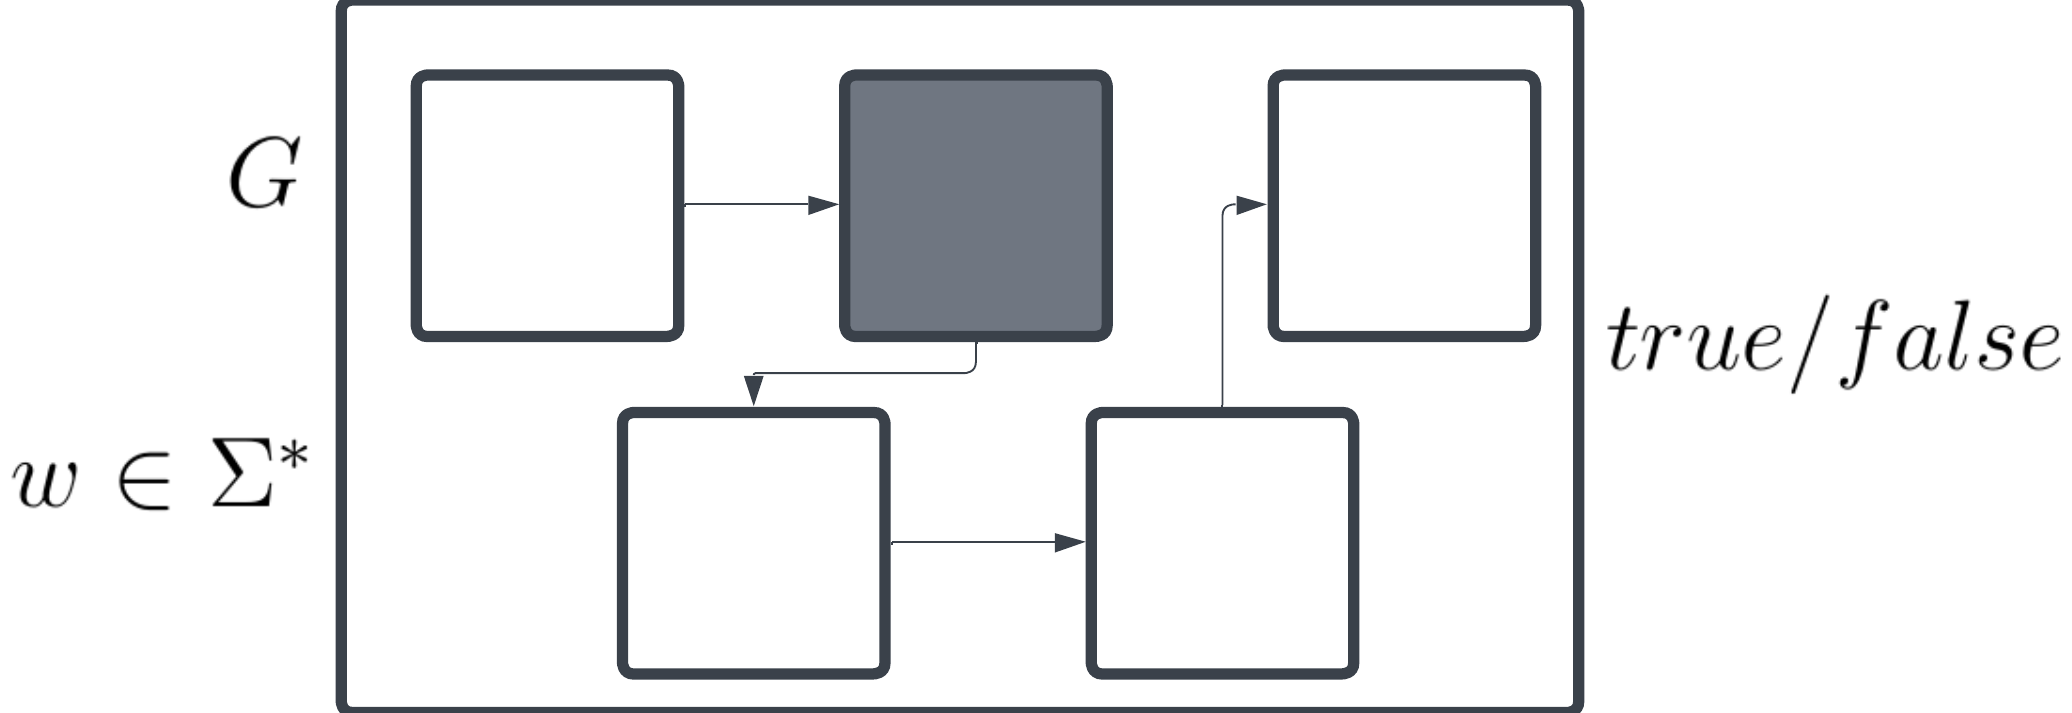
\includegraphics[width=12cm,height=4cm]{img/LGVT}
		\end{figure}
	\end{frame}

	\begin{frame}{Preparation}
		Die Definition der Matrixmultiplikation lautet folglich $c = a \cdot b$
		$$\textcolor{blue}{c_{ik}} = \textcolor{green}{a_{i1}} \cdot \textcolor{red}{b_{1k}} \cup \ldots \cup \textcolor{green}{a_{in}} \cdot \textcolor{red}{b_{nk}} =  \bigcup_{j=1}^{n} a_{ij} \cdot b_{ik}$$
		Sei A eine Matrize mit Einträgen $a_{ij} \subseteq N$
		die transitive Hülle einer quadratischen Matrize
		$$a^+ = a^{(1)} \cup a^{(2)} \cup \ldots$$
		Dabei wird $a^{(i)}$ wie folgt definiert:
		$$a^{(i)} = \bigcup_{j=1}^{i-1} a^{(j)} \cdot a^{(i-j)} \  und \ a^{(1)} = a$$
		die transitive Hülle für die Matrize $a$ endlich ist
	\end{frame}

	\begin{frame}{Preparation}
		ein Hemiring $(H, \cup, \emptyset,\cdot)$
		\begin{itemize}
			\item $H$ ist die Potenzmenge von $N$,
			\item $\cup$ ist die Vereinigung der Teilmengen von $N$. Dabei ist $\cup$ sowohl kommutativ als auch assoziativ,
			\item $\cdot$ ist die binäre Operation aus den Folien in CYK-Algorithmus und dabei $\cdot$ weder kommutativ noch assoziativ,
			\item $\emptyset$ ist das Nullelement eines Hemirings, d. h.
			\begin{itemize}
				\item $\emptyset$ ist neutrales Element bezüglich dem Operator $\cup$ d .h. \\
				$\emptyset \cup a = a \cup \emptyset = a \ f\ddot{u}r \ alle \ a\in H$, 
				\item $\emptyset$ ist absorbierend bezüglich dem Operator $\cdot$ d. h. \\
				$\emptyset \cdot a = a \cdot \emptyset = \emptyset \ f\ddot{u}r \ alle \ a\in H$.
			\end{itemize}
			$M(n)$ für das Problem der Multiplikation von $n\times n$ Matrizen, $T(n)$ für das Finden der transitiven Hülle von $n  \times n$ oberen Dreiecksmatrizen und $BM(n)$ für das Multiplizieren von $n \times n$ booleschen Matrizen. 
		\end{itemize}
	\end{frame}

	\begin{frame}{Wortproblem für CFL $\le$ Transitive Hülle}
		Sei $G = (S, \Sigma, N, P)$ eine kontextfreie Grammatik und $w=w_1 w_2 \ldots w_n$ ein Wort über $\Sigma^*$.
		Nun wird eine $(n+1)\times (n+1)$ obere Dreieckmatrix $b$ gebildet und wie folgt definiert:
		$$b_{i,i+1} = \{ A | A\to w_i \in P\} \ und \ b_{i,j}= \emptyset \ f\ddot{u}r \ alle \ j \neq i+1$$
		Aus der Definition der Multiplikationsoperation ergibt sich induktiv, dass die
		Elemente der transitiven Hülle $b^+$ ausschließlich diejenigen sind, die die Eigenschaft haben, dass 
		$$A \in b_{i,j}^+ \Leftrightarrow A \to^* w_i \ldots w_{j-1}$$
		Es kann also festgestellt werden, ob $S \to^* w$, indem $a = b^+$ berechnet und
		gefragt wird, ob $S \in a_{1,n+1}$ .
	\end{frame}

	\begin{frame}{Preparation}
		Somit ist die Reduktion korrekt, da das Wort $w$ vom Startsymbol $S$ genau dann abgeleitet wird, wenn das Startsymbol $S$ in dem oberen rechten Eintrag $a_{1,n+1}$ der Matrize $b^+$ zu finden ist. Unter Berücksichtigung des Aufwands für die Erstellung der oberen Dreieckmatrix $b$ entsteht die folgende Zeitkomplexität.
		\begin{block}{Theorem}
			$R(n) \le T(n+1) + O(n^2)$
		\end{block}
	\end{frame}

	\begin{frame}{Transitive Hülle $\le$ Multiplikation}
		\begin{block}{Lemma}
			Sei $b$ eine obere Dreieckmatrix der Größe $n \times n$
			und es wird angenommen, dass für einige $r > \dfrac{n}{2}$ der transitiven Hülle der Partitionen $[1\le i,j\le r]$ und $[n-r < i,j\le n]$ bekannt sind. Dann kann der Abschluss von b wie folgt berechnet werden:
			\begin{enumerate}
				\item Durchführung einer einzigen Matrixmultiplikation und
				\item finde die transitive Hülle von $2(n-r) \times 2(n-r)$ der oberen Dreieckmatrix, von der
				die Hülle der Partitionen $[1\le i,j\le n-r]$ und $[n-r < i,j\le 2(n-r)]$ bekannt sind.
			\end{enumerate}
		\end{block}
	
	\end{frame}

	\begin{frame}{Transitive Hülle $\le$ Multiplikation}
		Da die binäre Operation $\cdot$ nicht assoziativ ist, ist die Reihenfolge der Zusammensetzung von Matrixelementen wichtig. Die Matrixelemente haben die folgende Form:
		$$b_{i_1 i_2},\ b_{i_2 i_3},\ \ldots,\ b_{i_2 i_{t+1}} \ \ \ dabei \ u > v \Rightarrow  i_u > i_v$$
		Dies wird als ein $(i_1,i_{t+1})$-Term mit $t$ Komponenten bezeichnet. Zum Beispiel ist $(b_{2,5}\cdot (b_{5,7}\cdot b_{7,8}))\cdot b_{8,11}$ ein $(2, 11)$-Term mit vier Komponenten.
		Aus den getroffenen Annahmen geht klar hervor, dass der einzige Teil von $b^+$, der berechnet werden muss, die obere rechte Partition ist, d. h. $[1  \le i \le n-r; r< j \le n]$. Zunächst ist festzustellen, dass es in jedem $(k, 1)$-Term mit $k \le n-r$ und $l > r$ einen eindeutigen minimalen Unterterm gibt, der selbst ein $(p, q)$-Term mit $p \le n-r$ und $q   > r$ ist. Aber jeder dieser minimalen Teilterme hat entweder nur eine Komponente, den $(p,q)$-Term, oder ist die Zusammensetzung eines $(p, s)$-Terms mit einem $(s, q)$-Term, wobei gilt, dass $n-r< s \le r$. Die Vereinigung aller möglichen formal verschiedenen minimalen $(p,q)$-Unterterme ist also gegeben durch:
		$$b_{pq} \cup \bigcup_{n-r < s \le r}^{} b_{ps}^+ \cdot b_{sq}^+$$
	\end{frame}
	
	\begin{frame}{Transitive Hülle $\le$ Multiplikation}
		Aber $b_{ps}^+$ und $ b_{sq}^+$ sind durch die Annahme bekannt, dass $n-r< s\le r$. Somit werden die Partitionen $[1 \le i \le n-r;n-r < j \le r]$ und $[n-r < i \le r;r < j \le n]$ von $b^+$ mit einander multipliziert, dann wird die vorige Multiplikation mit der Partition $[1 \le i \le n-r; r < j \le n]$ von $b$ vereinigt. Somit entsteht eine $(n-r) \times (n-r)$-Matrix $c$ derart, dass $c_{p,q-r}$ gleich der Vereinigung aller formal verschiedenen minimalen $(p, q)$-Terme von $b$ ist.
			\begin{algorithm}[H]
			\floatname{algorithm}{Algorithmus}
			\setstretch{1.1}
			\caption{Lemma Teil 1}
			\label{algorithm12}
			\begin{algorithmic}[1]
				\Require $(b, r)$
				\State $b_{p,s} = b[1 \le i \le n-r;n-r < j \le r]$
				\State $b_{s,q} = b[n-r < i \le r;r < j \le n]$
				\State $b_{p,q} = b[1 \le i \le n-r; r < j \le n]$
				\State $c^{'} = b_{p,s} \cdot b_{s,q} = theorem3(b_{p,s},b_{s,q})$
				\State $c = c^{'} \cup b_{p,q}$
				\algstore{t}
			\end{algorithmic}
		\end{algorithm} 
	\end{frame}

	\begin{frame}{Transitive Hülle $\le$ Multiplikation}
			\begin{algorithm}[H]
			\addtocounter{algorithm}{-1}
			\caption{Lemma Teil 2}
			\begin{algorithmic}[1]
				\algrestore{t}
				\State $d = b$
				\State Ersetze den oberen rechten Teil von $d$ durch $c$.
				\State $d[1 \le i \le n-r; r < j \le n] = c$
				\State Eliminiere alle $i$-ten Zeilen und $i$-ten Spalten für $n-r < i \le r$.
				\State $d_{partition_1} = d[1 \le i \le n-r; 1 < j \le n-r]$
				\State $d_{partition_2} = d[1 \le i \le n-r; r < j \le n]$
				\State $d_{partition_3} = d[r \le i \le n; 1 < j \le n-r]$
				\State $d_{partition_4} = d[r \le i \le n; r < j \le n]$
				\State $d = 	
				\begin{bmatrix}
					d_{partition_1} & d_{partition_2}\\
					d_{partition_3} & d_{partition_4}
				\end{bmatrix}$
				\State Berechne die transitive Hülle von $d$.
				\State $theorem2(d)$
				\State Kopiere den oberen rechten Teil von $d$ in $b$.
				\State $b[1 \le i \le n-r; r < j \le n] = d[1 \le i \le n-r; n-r < j \le 2*(n-r)]$
			\end{algorithmic}
		\end{algorithm} 
	\end{frame}

	\begin{frame}{Transitive Hülle $\le$ Multiplikation}
		\begin{block} {Theorem}
				Sei $M(n)$ die Zeitkomplexität eines Matrixmultiplikationsalgorithmus
			der sich gut verhält in dem Sinne, dass es Konstanten $\gamma  \ge 2$ und $\iota   > 0$ gibt, so dass für alle m gilt,
			$$2^\gamma \cdot M(2^m) \le M(2^m)$$
			und für alle $\rho$, so dass $0 \le \rho < 2^m$,
			$$M(2^{m+1}) \le \iota \cdot M(2^m + \rho)$$
			Dann gibt es einen Algorithmus für das Berechnen der transitiven Hülle mit der der Komplexität T(n), so dass
			$$T(n) \le M(n) \cdot f(n)$$
			wobei $f(n)$ eine konstante Funktion ist, falls für einige $\gamma  > 2$ gilt. Außerdem ist in jedem Fall $f(n) = O(\log n)$. 
		\end{block}
	\end{frame}

	\begin{frame}{Transitive Hülle $\le$ Multiplikation}
		Beweis. Wenn $b$ eine $n \times n$ obere Dreieckmatrix ist, wird mit $P_k$ die Operation
		bezeichnet, die ihre Hülle finden soll, wenn jene ihrer Partitionen $[1 \le i, j \le n - \dfrac{n}{k}]$ und $[\dfrac{n}{k} < i, j \le n]$ bereits bekannt sind. Diese Aufgaben für $k = 2,\ 3$ und $4$ können rekursiv
		wie folgt definiert werden:
		\begin{algorithm}[H]
			\floatname{algorithm}{Algorithmus}
			\setstretch{1.1}
			\caption[P2]{P2}
			\label{algorithm14}
			\begin{algorithmic}[1]
				\Require $(b)$
				%			\State $n = len(b)$
				%			\If{$n < 4$}
				%			\State Tue Nichts.
				%			\EndIf
				\State $P2(b[\dfrac{n}{4} < i, j\le \dfrac{3n}{4}])$ Anwendung von $P_2$ auf die eingegebene Partition.
				\State $P3(b[1 \le i, j\le \dfrac{3n}{4}])$ Anwendung von $P_3$ auf die eingegebene Partition.
				\State $P3(b[\dfrac{n}{4} < i, j\le n])$ Anwendung von $P_3$ auf die eingegebene Partition.
				\State $P4(b)$ Anwendung von $P4$.
			\end{algorithmic}
		\end{algorithm} 
	\end{frame}

	\begin{frame}{Transitive Hülle $\le$ Multiplikation}
		\begin{algorithm}[H]
			\floatname{algorithm}{Algorithmus}
			\setstretch{1.1}
			\caption[P3]{P3}
			\label{algorithm15}
			\begin{algorithmic}[1]
				\Require $(b)$
				%			\State $n = len(b)$
				%			\If{$n < 3$}
				%			\State Tue Nichts.
				%			\EndIf
				\State $lemma(b, r = \dfrac{2n}{3})$ Anwendung von dem Verfahren des Lemmas für $r = \dfrac{2n}{3}$.
			\end{algorithmic}
		\end{algorithm} 
		
		\begin{algorithm}[H]
			\floatname{algorithm}{Algorithmus}
			\setstretch{1.1}
			\caption[P4]{P4}
			\label{algorithm16}
			\begin{algorithmic}[1]
				\Require $(b)$
				%			\State $n = len(b)$
				%			\If{$n < 4$}
				%			\State Tue Nichts.
				%			\EndIf
				\State $lemma(b, r = \dfrac{3n}{4})$ Anwendung von dem Verfahren des Lemmas für $r = \dfrac{3n}{4}$.
			\end{algorithmic}
		\end{algorithm} 
	\end{frame}

	\begin{frame}{Transitive Hülle $\le$ Multiplikation}
			Wenn $T_i(n)$ die Zeitschranke der Prozedur $P_i$ bei Anwendung auf eine $n \times n$-Matrix ist, ergibt das die drei folgenden Zeitschranken:
		$$T_2(n) = T_2(\dfrac{n}{2}) + 2T_3(\dfrac{3n}{4}) + T_4(n),$$
		$$T_3(n) = M(\dfrac{n}{3}) + T_2(\dfrac{2n}{3}) + O(n^2),$$
		$$T_4(n) = 2M(\dfrac{n}{4}) + T_2(\dfrac{n}{2}) + O(n^2).$$
		Werden $T_3$ und $T_4$ in $T_2$ ersetzt, so ergibt sich, dass
		$$T_2(n) = 4T_2(\dfrac{n}{2}) + 4M(\dfrac{n}{4}) + O(n^2).$$
		Da $M(2^{m+1}) \ge 2^\gamma \cdot M(2^m)$, wenn $n$ eine Potenz von $2$ ist, dann
		$$T_2(n) \le O(n^2 \log n) + 4M(\dfrac{n}{4}) \cdot \sum_{m=0}^{\log n} 2^{(2-\gamma)m}.$$
		Aber $\sum_{m=0}^{\infty }$ konvergiert, wenn $|x| < 1$. Wenn also $\gamma  > 2$, 
		$$T_2(n) \le M(n) \cdot Konstante$$
		Wenn $\gamma = 2$, dann $T_2(n) \le M(n) \cdot \log n \cdot Konstante$\\
		Der Abschluss von $b$ kann berechnet werden, indem wir die Partitionen $[1 \le i,j\le \dfrac{n}{2}]$ und $[\dfrac{n}{2} < i, j \le n]$ schließen, und dann $P_2$ darauf anwenden. Dies ergibt:
		$$T(n) = 2T(\dfrac{n}{2}) + T_2(n) + O(n^2).$$
	\end{frame}

	\begin{frame}{Transitive Hülle $\le$ Multiplikation}
		Es wurde laut \cite{booleanmatrix} beobachtet, dass der Abschluss einer booleschen Matrix der Größe $3n \times 3n$, die überall null bzw. $\emptyset$ als Einträge enthält, mit Ausnahme der Partitionen $[1 \le i \le n; n < j \le 2n]$ und $[n < i \le 2n; 2n < j \le 3n]$, das Produkt dieser Teilungen ergibt. Dies gilt auch hier eindeutig und liefert eine umgekehrte Ungleichung der Form.
		$$M(n) \le T(3n) + O(n^2)$$
		Somit unterscheiden sich innerhalb einer allgemeinen Klasse von Operationen die Komplexität der Berechnung von Matrixprodukten von der transitiven Hülle jeweils um höchstens einen logarithmischen Faktor.
	\end{frame}

	\begin{frame}{Multiplikation $\le$ Boolesche Multiplikation}
		\begin{block}{Theorem}
			$M(n) \le BM(n) \cdot Konstante$
		\end{block}
		Beweis. Sei $G = (S, \Sigma, N, P)$ eine Kontextfreie Grammatik und seien $a$ und $b$ zwei $n \times n$ Matrizen mit $a_{ij},b_{ij}\subseteq N$ für $i,j\in\{1,\ldots ,n\}$
		$$c = a\cdot b$$
		$2|N|$ booleschen Matrizen $a[N_i], b[N_i]$ für $i=1,\ldots,|N|$ mit $N_i$ bzw. $i$-ten nichtterminalen Zeichen 
		$$a[N_i]_{jk} = 1 \ falls \ N_i \in a_{jk}, \ \ \ \ \ b[N_i]_{jk} = 1 \ falls \ N_i \in b_{jk}$$
		Für jedes Paar $N_i,\ N_j$ wird dann die boolesche Matrix $c[N_i, N_j]$ für $i.j \in \{1,\ldots,|N|\}$ berechnet, wobei
		$$c[N_i,\ N_j] = a[N_i] \times b[N_j]$$
		Dies erfordert ${|N|}^2$ boolesche Matrixmultiplikationen. Offensichtlich kann $c$ dann direkt erhalten werden, da nach der Konstruktion $N_k \in c_{ij} \ falls$
		$$\exists N_i,\ N_j \ so dass, \ c[N_i,\ N_j] = 1 \ and\ N_k \to N_i N_j  \in P$$
	\end{frame}

	\begin{frame}{Zusammenfassung}
			\begin{figure}
			\centering
			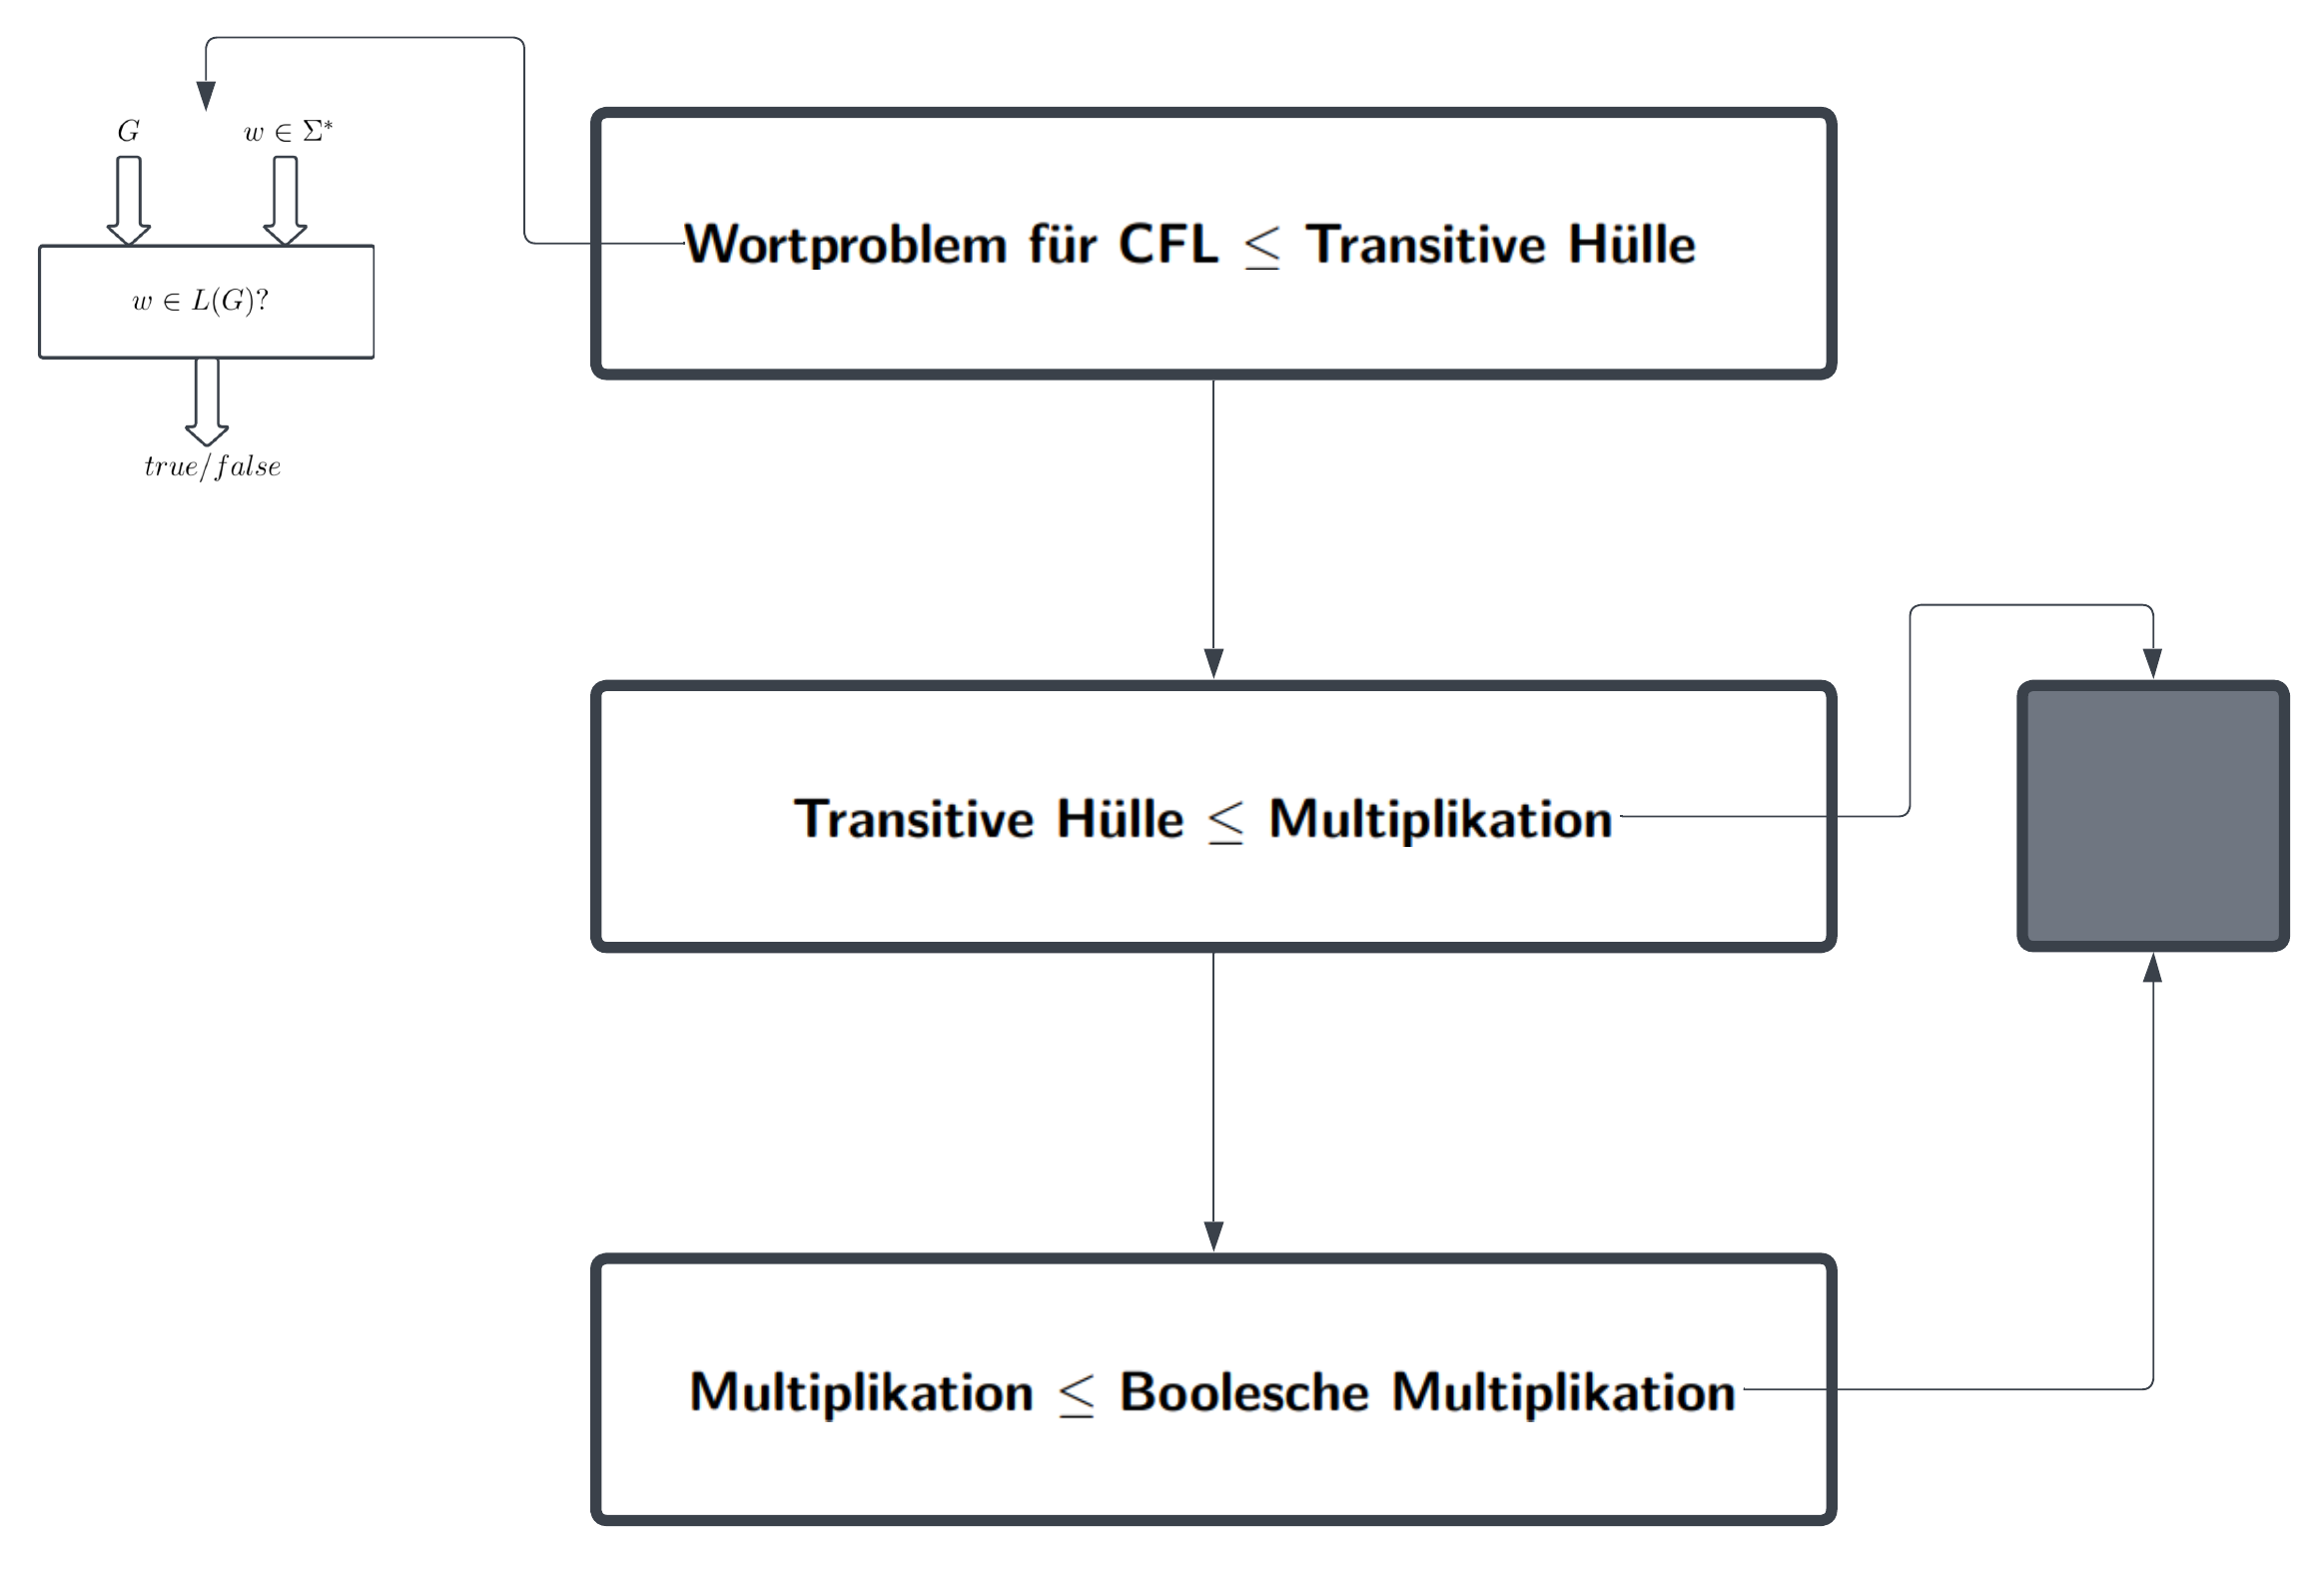
\includegraphics[width=10.5cm,height=7.5cm]{img/ZusammenfassungT}
		\end{figure}
	\end{frame}
	

	%---------------------------------------------------------
	
	
	
	
	\section{Boolesche-Strassen-Matrix-Multiplikation}

	\begin{frame}{Strassen-Matrix-Multiplikation}
		Seien A und B zwei $2 \times 2$ Matrizen 
		$$
		\begin{bmatrix}
			a_{11} & a_{12}\\
			a_{21} & a_{22} 
		\end{bmatrix}
		\times
		\begin{bmatrix}
			b_{11} & b_{12}\\
			b_{21} & b_{22}
		\end{bmatrix}
		=
		\begin{bmatrix}
			a_{11} b_{11}  + a_{12} b_{21} & a_{11} b_{12} + a_{12} b_{22}\\
			a_{21} b_{11} + a_{22} b_{21} & a_{21} b_{12} + a_{22} b_{22}
		\end{bmatrix}
		$$
		
		$$
		\begin{bmatrix}
			a_{11} & a_{12}\\
			a_{21} & a_{22} 
		\end{bmatrix}
		\times
		\begin{bmatrix}
			b_{11} & b_{12}\\
			b_{21} & b_{22}
		\end{bmatrix}
		=
		\begin{bmatrix}
			M_{1} + M_{2} - M_{4} + M_{6} & M_{4} + M_{5}\\
			M_{6} + M_{7} & M_{2} - M_{3} + M_{5} - M_{7}
		\end{bmatrix}
		$$
		
		$$ M_{1} = (a_{12} - a_{22}) \cdot (b_{21} + b_{22}) $$
		$$M_{2} = (a_{11} + a_{22}) \cdot (b_{11} + b_{22}) $$
		$$M_{3} = (a_{11} - a_{21}) \cdot (b_{11} + b_{12})$$
		$$M_{4} = (a_{11} + a_{12}) \cdot b_{22}$$
		$$M_{5} = a_{11} \cdot (b_{12} - b_{22})$$
		$$M_{6} = a_{22} \cdot (b_{21} - b_{11})$$
		$$M_{7} = (a_{21} + a_{22}) \cdot b_{11}$$
	\end{frame}


	\begin{frame}{Strassen-Matrix-Multiplikation}
		Seien A und B zwei $n \times n$ Matrizen als Eingabe für den folgenden Algorithmus
		\begin{algorithm}[H]
			{Algorithmus}
			\setstretch{1.1}
			\caption[Strassen-Matrix-Multiplikation]{Strassen-Matrix-Multiplikation}
			\begin{algorithmic}[1]
				\Require $(A, \ B)$
				\Ensure $A \times B$
				\If{$length(A) = 1, 2, 4, 8, 16, n^2$}  \ \ \ \ \ \ \ \ \ \ \ \ \ \ \ \ \ \ \ \ \ \ \ \ \ \ \ \ \ \ \ \ \ \ \textbf{\{Basisfall\}}
				\State $A \times B$
				\Else  \ \ \ \ \ \ \ \ \ \ \ \ \ \ \ \ \ \ \ \ \ \ \ \ \ \ \ \ \ \ \ \ \ \ \ \ \ \ \ \ \ \ \ \ \ \ \ \ \ \ \ \ \ \ \ \ \ \ \ \textbf{\{rekursiver Fall\}}
				\State $$
				\begin{bmatrix}
					A_{11} \vline A_{12}\\ \hline
					A_{21} \vline A_{22} 
				\end{bmatrix}
				\times
				\begin{bmatrix}
					B_{11} \vline B_{12}\\ \hline
					B_{21} \vline B_{22}
				\end{bmatrix}
				=
				\begin{bmatrix}
					C_{11} \vline C_{12}\\ \hline
					C_{21} \vline C_{22}
				\end{bmatrix}
				$$
				
				\algstore{t}
			\end{algorithmic}
		\end{algorithm} 
	\end{frame}

	\begin{frame}{Strassen-Matrix-Multiplikation}
		\begin{algorithm}[H]
			\floatname{algorithm}{Algorithmus}
			\setstretch{1.1}
			\caption[Strassen-Matrix-Multiplikation]{Strassen-Matrix-Multiplikation}
			\begin{algorithmic}[1]
				\algrestore{t}
				\State $m_1$ = Strassen-Matrix-Multiplikation($(a_{12} - a_{22}) ,\ (b_{21} + b_{22})$)
				\State $m_2$ = Strassen-Matrix-Multiplikation($(a_{11} + a_{22}) ,\ (b_{11} + b_{22})$)
				\State $m_3$ = Strassen-Matrix-Multiplikation($(a_{11} - a_{21}) ,\ (b_{11} + b_{12})$)
				\State $m_4$ = Strassen-Matrix-Multiplikation($(a_{11} + a_{12}) ,\ b_{22}$)
				\State $m_5$ = Strassen-Matrix-Multiplikation($a_{11} ,\ (b_{12} - b_{22})$)
				\State $m_6$ = Strassen-Matrix-Multiplikation($a_{22} ,\ (b_{21} - b_{11})$)
				\State $m_7$ = Strassen-Matrix-Multiplikation($(a_{21} + a_{22}) ,\ b_{11}$)
				\State $c_{11} = m_{1} + m_{2} - m_{4} + m_{6}$
				\State $c_{12} = m_{4} + m_{5}$
				\State $c_{21} = m_{6} + m_{7}$
				\State $c_{22} = m_{2} - m_{3} + m_{5} - m_{7}$
				\State return 
				$\begin{bmatrix}
					C_{11} & C_{12}\\
					C_{21} & C_{22}
				\end{bmatrix}$
				\EndIf
			\end{algorithmic}
		\end{algorithm} 
	\end{frame}
		
	
	\begin{frame}{Zeitkomplexität für Strassen}
		
		Sei $T_M(n)$ bzw. $T_A(n)$ die Anzahl der Multiplikationen und Additionen
		$$
		T_M(n) = 
		\begin{cases}
			1, & n=1\\
			7 \cdot T_M(n \textfractionsolidus 2), & n>1 
		\end{cases}
		$$
		Daraus kann abgeleitet werden, dass:
		$$T_M(n) = \underbrace{7 \cdot 7 \ldots 7}_{(\log n)-mal} = 7^{\log n} = n^{\log 7} \le n^{2.8074}$$
		\\
		Für $T_A(n)$ gilt:
		$$
		T_A(n) = 
		\begin{cases}
			0, & n=1\\a
			18(n\textfractionsolidus 2) (n\textfractionsolidus 2) + 7T_A(n\textfractionsolidus 2), & n>1 
		\end{cases}
		$$
		Dadurch wird $T_A(n) = O(n^{2.8074})$ erhalten.
	\end{frame}	


	\begin{frame}{Strassen für Boolesche Matrizen}
		Für die schulische Matrix-Multiplikation könnte die boolesche dafür so aussehen:
		\pause
		$$c_{ij} = \lor_{k=1}^n a_{ik}\land b_{kj} $$
		\pause
		Jedoch ist diese Formel nicht ausreichend für Strassen, da deren Berechnung auch noch Subtraktion
		\begin{itemize}
			\item Die boolesche Matrix-Multiplikation kann durch die integer Matrix-Multiplikation simuliert werden. Wenn die Multiplikation zu Ende ist, dann werden die $0$-Einträge der Matrize $C$ durch $0$ und alle anderen Einträge durch $1$ ersetzt.
			\item Eine andere Methode für boolesche Matrixmultiplikationen verwendet nur Bit-Operationen und setzt auch Randomisierung ein. Hierbei werden logisches $and$ und $or$ durch Multiplikation und Addition modulo 2 ersetzt.
		\end{itemize}
		
	\end{frame}

	\begin{frame}{Zeitkomplexität für oolesche Strassen}
		\begin{algorithm}[H]
			\floatname{algorithm}{Algorithmus}
			\setstretch{1.1}
			\caption[Boolean-Strassen]{Boolean-Strassen}
			\label{algorithm20}
			\begin{algorithmic}[1]
				\Require $(A, \ B)$
				\Ensure $A \times B$
				\State $c$ = Strassen-Matrix-Multiplikation-Algorithmus$(A ,\ B$) \textbf{$ \%O(n^{2.8074})$ Zeit}
				\State $c \ ist \ eine \ n \times m \ Matrix$
				\For{\texttt{$i:=1 \ to \ n$}} \ \ \ \ \ \ \ \ \ \ \ \ \ \ \ \ \ \ \ \ \ \ \ \ \ \ \ \ \ \ \ \ \ \ \ \ \ \textbf{$ \%O(n)$ Durchläufe}
				\For{\texttt{$j:=1 \ to \ m$}} \ \ \ \ \ \ \ \ \ \ \ \ \ \ \ \ \ \ \ \ \ \ \ \ \ \ \ \ \ \ \ \textbf{$ \%O(m)$ Durchläufe}
				\If{$c[i][j] \neq 0$}
				\State $c[i][j] = 1$
				\EndIf
				\EndFor
				\EndFor
				\State return $c$
			\end{algorithmic}
		\end{algorithm}
	\end{frame}

	\begin{frame}[plain]
		\begin{table}[H]
			\centering
			\begin{tabular}{|m{2cm}||m{2.5cm}|m{2.5cm}|m{2.5cm}|} 
				\hline
				\diagbox[width=\dimexpr \textwidth/8+3\tabcolsep\relax, height=1cm]{}{}& $1000\times 1000$ & $2000\times2000$ & $4000\times4000$ \\ [0.5ex] 
				\hline\hline
				$n=1$ & $3918.410s$ & $27363.411s$ & $100\ldots00 s$\\[1ex]
				\hline
				$n=2$ & $774.119s$ & $5483.681s$ & $100\ldots00 s$\\[1ex]
				\hline
				$n=4$ & $117.295s$ & $823.133s$ & $5770.478s$\\[1ex]
				\hline
				$n=8$ & $21.732s$ & $145.509s$ & $967.924s$\\[1ex]
				\hline
				$n=16$ & $6.765s$ & $36.112s$ & $216.553s$\\[1ex]
				\hline
				$n=32$ & $3.905s$ & $19.076s$ & $93.765s$\\[1ex]
				\hline
				$n=64$ & $3.606s$ & $14.754s$ & $68.552s$\\[1ex]
				\hline
				$n=128$ & $3.466s$ &$14.826s$ &$63.704s$\\[1ex]
				\hline
				$n=256$ & $3.167s$ & $13.505s$ &$58.498s$\\[1ex]
				\hline
				$n=512$ & $3.244s$ & $12.964s$ & $54.527s$\\[1ex]
				\hline
				$n=1024$ & $3.891s$ & $12.716s$ & $52.362s$\\[1ex]
				\hline
				$n=2048$ & $3.817s$ & $34.466s$ & $51.265s$\\[1ex]
				\hline
			\end{tabular}
		\end{table}
	\end{frame}
	
	\section{Zeitergebnisse}
	
	\begin{frame}{CYK-Algorithmus vs. LGV-Algorithmus}
		1. Test: Grammatiken mit einem nichtterminalen Zeichen und verschiedene Anzahl von Regeln
		\pause
		\begin{itemize}
			\item $G_1 = (S, \{a\}, \{S\}, \{S\to SS | a\})$
			\item $G_2 = (S, \{a,b,c,d\}, \{S\}, \{S\to SS | a | b | c |d\})$
		\end{itemize}
		\pause
		\begin{table}[H]
			\centering
			\begin{tabular}{|m{2cm}||m{1.7cm}|m{1.7cm}||m{1.7cm}|m{1.7cm}|} 
				\hline
				\multirow{2}{*}{\diagbox[width=\dimexpr \textwidth/8+4.5\tabcolsep\relax, height=1cm]{$|w|$}{$Grammatik$}}& \multicolumn{2}{c||}{$|N|=1 \ |P|=2$} & \multicolumn{2}{c|}{$|N|=1 \ |P|=5$}\\ [0.5ex] 
				\cline{2-5}
				& CYK & LGV & CYK & LGV\\
				\hline\hline
				$254$ & $9.429s$ & $14.008s$ &$10.658s$&$13.820s$\\[1ex]
				\hline
				$510$ & $82.134s$ & \cellcolor{lightgray}$81.0641s$ & $90.295s$&\cellcolor{lightgray}$79.939s$\\[1ex]
				\hline
				$1022$ & $649.915s$ & \cellcolor{green}$457.080s$ & $717.655s$&\cellcolor{green}$454.532s$\\[1ex]
				\hline
				$2046$ & $5192.263s$ & $2571.086s$ & $5740.248s$&$2585.514s$\\[1ex]
				\hline
				$4094$ & $41030.947s$ & $14531.633s$ & $48343.457s$&$14539.953s$\\[1ex]
				\hline
				$8190$ & $\ldots s$ & $\ldots s$ & $\ldots s$ & $\ldots s$ \\[1ex]
				\hline
			\end{tabular}
		\end{table}
	\end{frame}

	
	%---------------------------------------------------------
	
	\begin{frame}{CYK-Algorithmus vs. LGV-Algorithmus}
		2. Test: Grammatiken mit einem nichtterminalen Zeichen und verschiedene Anzahl von Regeln
		\pause
		\begin{itemize}
			\item $G_3 = (S, \{a,b\}, \{S,B\}, \{S\to SB | BS | a | b ,B\to b\})$
			\item $G_4 = (S, \{a,b\}, \{S,A,B\}, \{S\to SB | SA | a | b ,B\to b\ ,A\to a\})$
		\end{itemize}
		\pause
		\begin{table}[H]
			\centering
			\begin{tabular}{|m{2cm}||m{1.7cm}|m{1.7cm}||m{1.7cm}|m{1.7cm}|}  
				\hline
				\multirow{2}{*}{\diagbox[width=\dimexpr \textwidth/8+4.5\tabcolsep\relax, height=1cm]{$|w|$}{$Grammatik$}}& \multicolumn{2}{c||}{$|N|=2$}  & \multicolumn{2}{c|}{$|N|=3$}\\ [0.5ex] 
				\cline{2-5}
				& CYK & LGV & CYK & LGV \\
				\hline\hline
				$254$ & $10.382s$& $23.382s$&$12.145s$& $35.979s$\\[1ex]
				\hline
				$510$ & $86.694s$& $134.923s$& $97.738s$& $207.755s$\\[1ex]
				\hline
				$1022$ & $730.844s$& \cellcolor{lightgray}$771.789s$& $804.681s$& $1180.179s$\\[1ex]
				\hline
				$2046$ & $5706.038s$& \cellcolor{green}$4365.122s$&$6311.629s$& \cellcolor{lightgray}$6685.876s$\\[1ex]
				\hline
				$4094$ & $46464.972s$& $24703.334s$& $51015.653s$& \cellcolor{green}$37991.584s$\\[1ex]
				\hline
				$8190$ & $\ldots s$& $\ldots s$& $\ldots s$& $\ldots s$\\[1ex]
				\hline
			\end{tabular}
		\end{table}
	\end{frame}
	
	%---------------------------------------------------------
	
	\begin{frame}{CYK-Algorithmus vs. LGV-Algorithmus}
		3. Test: Grammatiken mit einem nichtterminalen Zeichen und verschiedene Anzahl von Regeln
		\pause
		\begin{itemize}
			\item $G_5 = (S, \{a,b\}, \{S,A,B,C\},$ \\ $ \{S\to AB | AC ,C\to SB,B\to b\ ,A\to a\})$
		\end{itemize}
		\pause
		\begin{table}[H]
			\centering
			\begin{tabular}{|m{2.5cm}||m{2cm}|m{2cm}|} 
				\hline
				\multirow{2}{*}{\diagbox[width=\dimexpr \textwidth/8+5.3\tabcolsep\relax, height=1.1cm]{$|w|$}{$Grammatik$}}& \multicolumn{2}{c|}{$|N|=4$}\\ [0.5ex] 
				\cline{2-3}
				& CYK & LGV \\
				\hline\hline
				$254$ & $12.120s$& $53.519s$\\[1ex]
				\hline
				$510$ & $99.725s$& $305.683s$\\[1ex]
				\hline
				$1022$ & $824.670s$& $1744.574s$\\[1ex]
				\hline
				$2046$ & $6353.308s$& $9999.785s$\\[1ex]
				\hline
				$4094$ & $51319.035s$& \cellcolor{lightgray}$55878.540s$\\[1ex]
				\hline
				$8190$ & $\ldots s$& \cellcolor{green}$\ldots s$\\[1ex]
				\hline
			\end{tabular}
		\end{table}
	\end{frame}
	
	%---------------------------------------------------------
	
	\begin{frame}{LGV-Algorithmus und $\#$ nichtterminalen Zeichen}
		Wie verhält sich LGV-Algorithmus im Bezug auf die Anzahl der nichtterminalen Zeichen für ein Wort der Länge $|w| = 4094$ 
		\pause
		\begin{figure}[H]
			\begin{tikzpicture}[scale=0.9]
				\begin{axis}[
					%		title={nothing},
					xlabel={Anzahl der nichtterminalen Zeichen $|N|$},
					ylabel={Zeit in Stunden},
					%			ymin=0, ymax=130,
					%			xmin=0, xmax=146,
					xtick={1,2,3,4,5},
					%			ytick={0,1,2,4,8,16,32,64,128,256},
					ymajorgrids=true,
					grid style=dashed,
					]
					
					\addplot[
					color=blue,
					mark=otimes*,
					]
					coordinates {
						(1,4.038)(2,6.862)(3,10.553)(4,15.521)
					};
					
					%			\legend{$CYK$,$LGV$}
				\end{axis}
			\end{tikzpicture}
			\centering
			\label{LGV Verhältnis bzgl. N}
		\end{figure}
	\end{frame}
	
	%---------------------------------------------------------
	
	\begin{frame}{Warum $|w| = 2^n-2$ und Was ist rein kontextfrei}
		\begin{itemize}
			\item Warum wurden die Wortlängen $|w| = 2^n-2$ für $n = 8,9,10,11,12$ und $13$ so gewählt?
			\pause
			\item Welche Sprachen erzeugen die Grammatiken $G_1, G_2, G_3, G_4$ und $G_5$? Sind diese Sprachen rein kontextfrei?
		\end{itemize}
		\pause
		\begin{figure}[H]
			\begin{tikzpicture}[scale=5]
				\node[above,ellipse,minimum height=4em,minimum width=4em,draw] (a) {Typ 3: Reguläre Sprachen};
				\node[above,ellipse,minimum height=7em,minimum width=20em,draw] (b) {};
				\node[above,ellipse,minimum height=10em,minimum width=25em,draw] (c) {};
				\node[above,ellipse,minimum height=13em,minimum width=30em,draw] (d) {};
				\path (a.north) node[above] {Typ 2: Kontextfreie Sprachen}
				(b.north) node[above] {Typ 1: Kontextsensitive Sprachen}
				(c.north) node[above] {Typ 0: Aufzählbare Sprachen};
			\end{tikzpicture}
			\label{Chomsky-Hierarchie}
		\end{figure}
	\end{frame}

	%---------------------------------------------------------
	
	\section{Zusammenfassung}
	
	\begin{frame}{Zusammenfassung}
		Wortproblem für kontextfreie Sprachen in subkubischer Zeit:
		\begin{itemize}
			\item Umwandlung von kontextfreien Grammatiken in Chomsky-Normalform.
			\pause
			\item CYK-Algorithmus hat die Zeitkomplexität $O(n^{3})$
			\pause
			\item LGV-Algorithmus hat die Zeitkomplexität $O(n^{2.81})$
			\pause
			\item Tests zwischen den beiden Algorithmen auf Uni-Cluster durchführen
			\pause
			\item Wählen von großen Wörtern der Länge zwischen $254$ und $8190$
			\pause
			\item Wählen Grammatiken mit unterschiedlichen Anzahl von nicht terminalen Zeichen
			\pause
			\item Tests haben gezeigt, dass CYK-Algorithmus wirklich schneller ist als LGV-Algorithmus
		\end{itemize}
	\end{frame}

	%---------------------------------------------------------
\end{document}